\renewcommand{\papertitle}{Preliminary coating design coating developments for ATHENA}
\chapter{\papertitle}
\label{pap:PREL_ATHENA}
\markboth{\appendixname\ \thechapter}{\papertitle}


Publication printed in {\em Proc.\ SPIE,\ Optics for EUV, X-Ray, Gamma-Ray Astronomy V}.

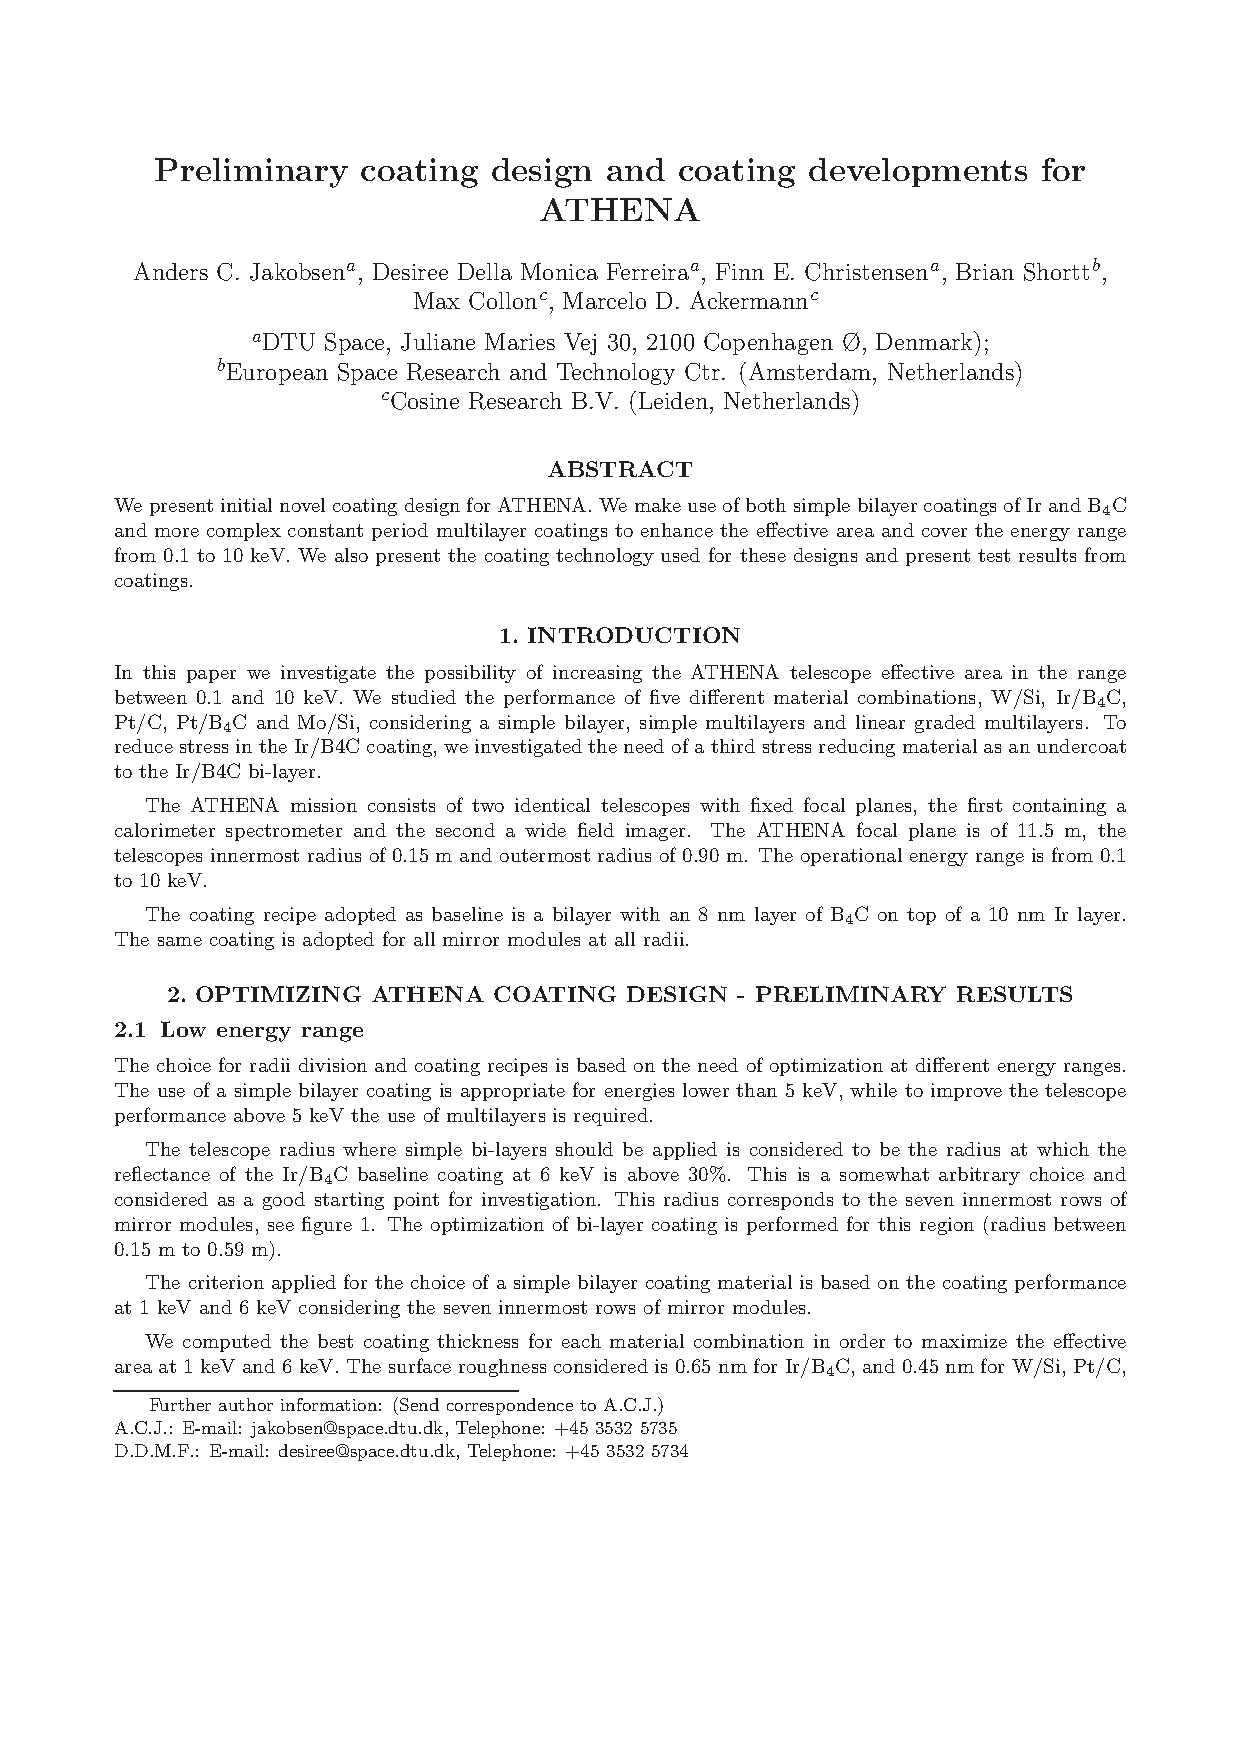
\includepdf[pages=-,scale=.9,pagecommand={}]{papers/prel_athena.pdf}

\newpage\mbox{} % Blank side s� artiklen starter p� et ulige sidetal
\markboth{}{}



\renewcommand{\papertitle}{X-ray optics for axion helioscopes}
\chapter{\papertitle}
\label{pap:axion_spie}
\markboth{\appendixname\ \thechapter}{\papertitle}

Publication printed in {\em Proc.\ SPIE,\ Optics for EUV, X-Ray, Gamma-Ray Astronomy VI}.
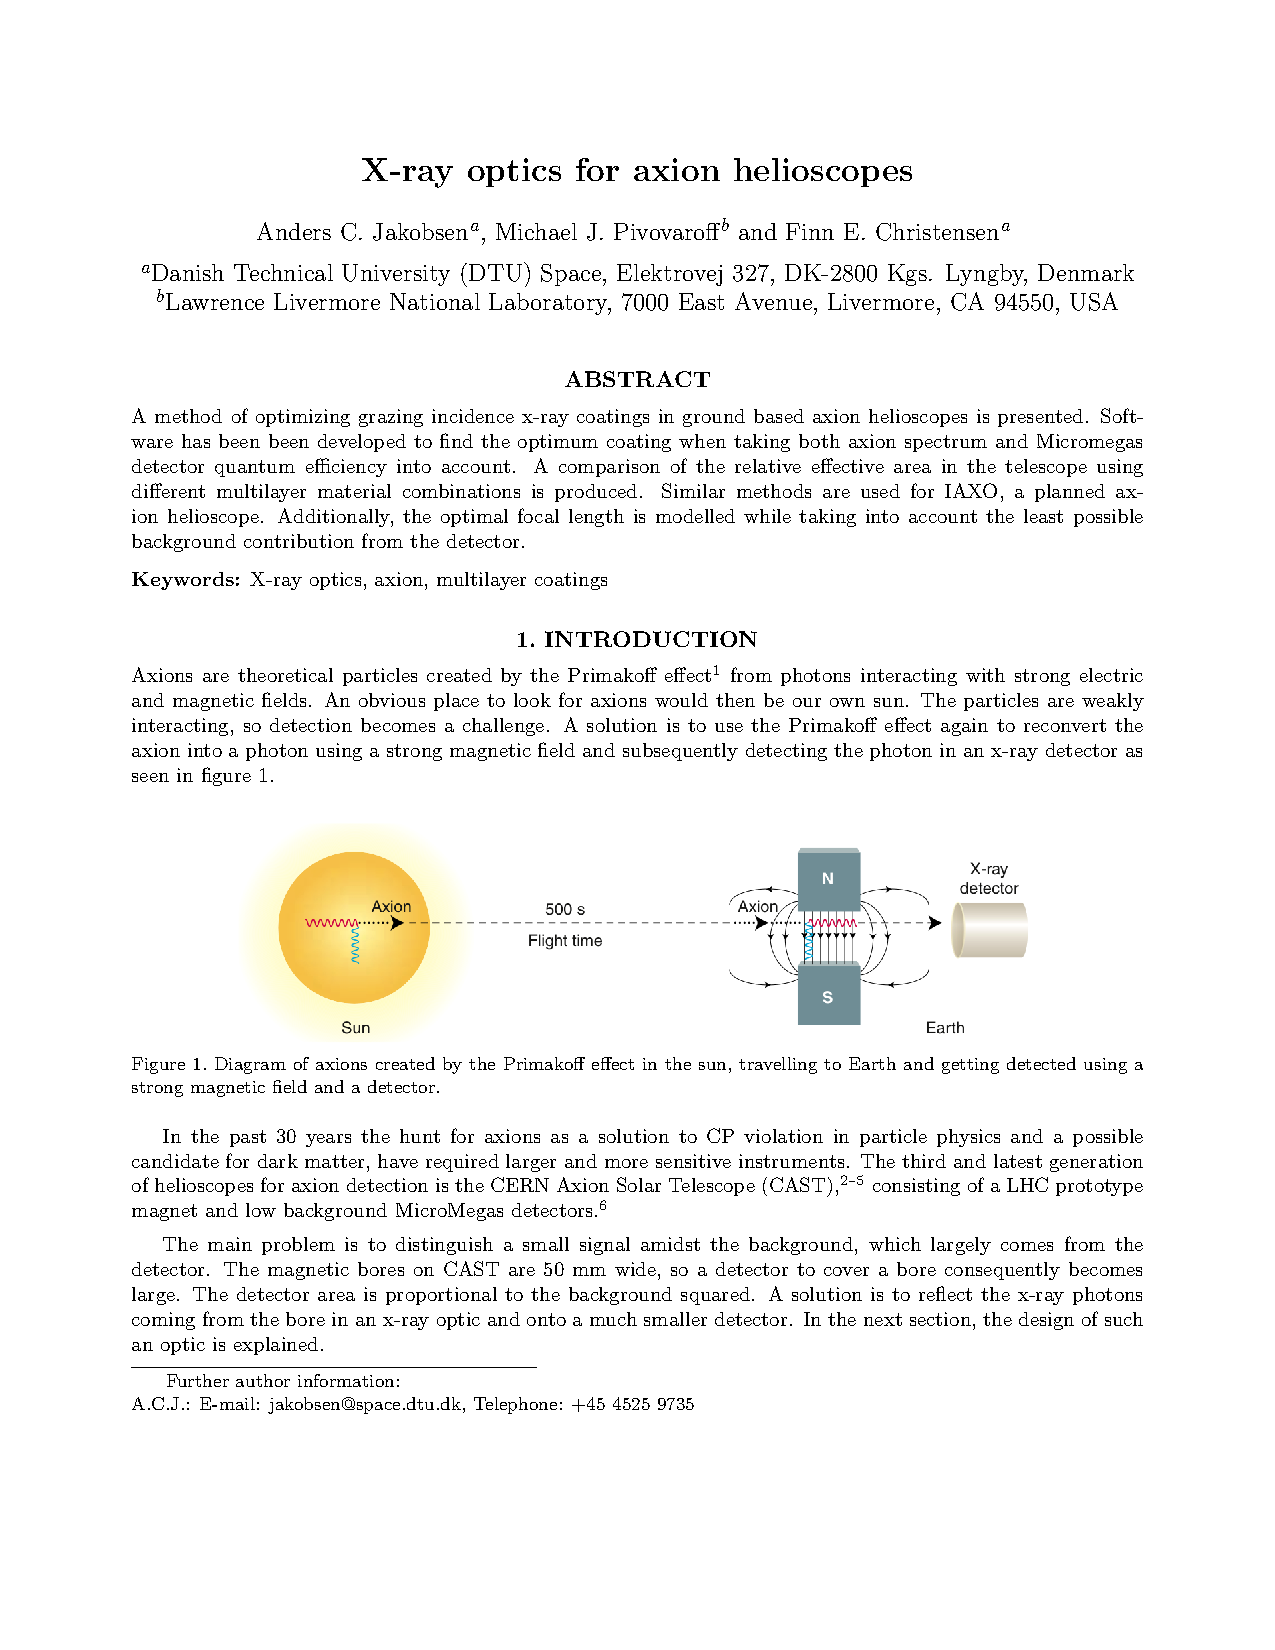
\includepdf[pages=-,scale=.9,pagecommand={}]{papers/axion_spie.pdf}

\newpage\mbox{} % Blank side s� artiklen starter p� et ulige sidetal
\markboth{}{}



\renewcommand{\papertitle}{Conceptual design of the International Axion Observatory (IAXO)}
\chapter{\papertitle}
\label{pap:iaxo_concept}
\markboth{\appendixname\ \thechapter}{\papertitle}

Publication printed in {\em Journal\ of\ Instrumentation}\\
\\
Presented in this thesis is a shorter version of the paper, only representing the work that I did. The full paper is 46 pages a large part is outside the field of X-ray optics.
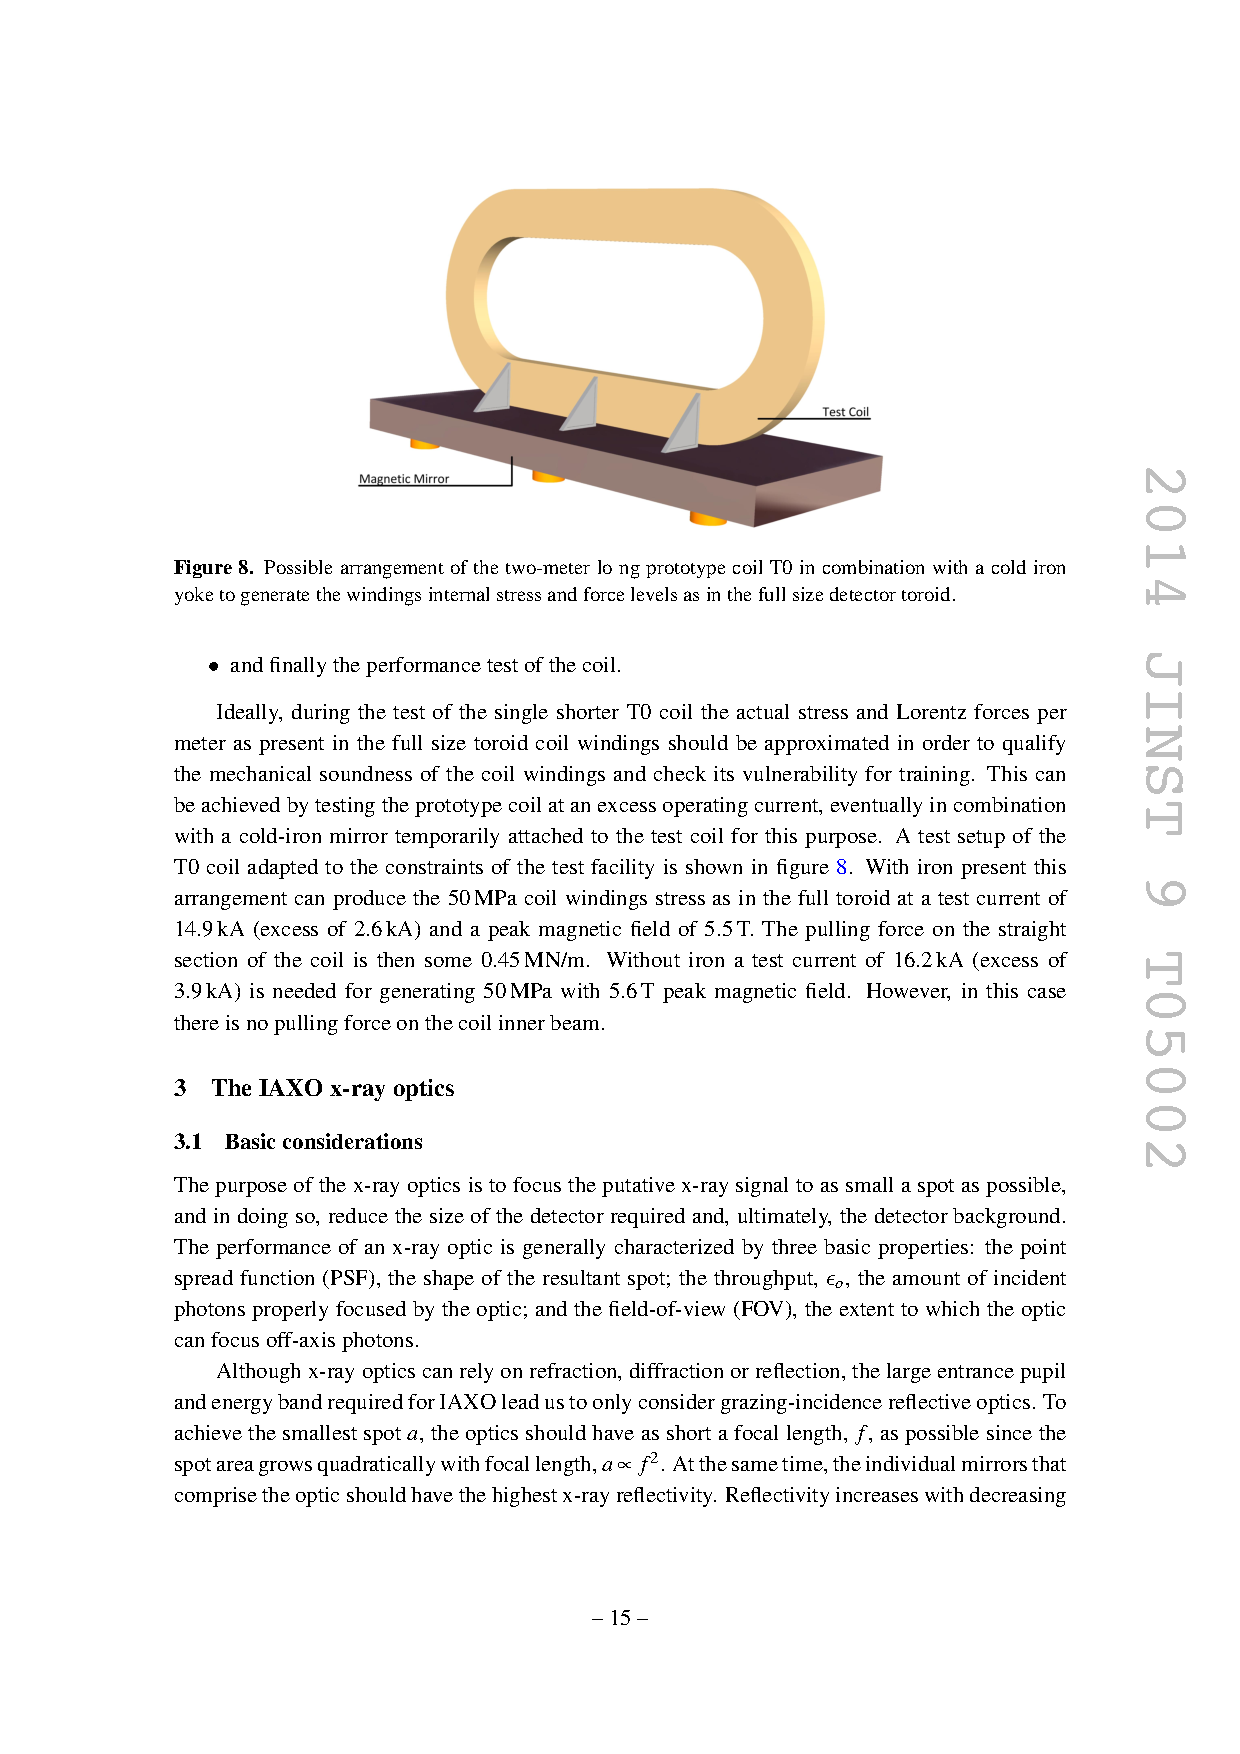
\includepdf[pages=-,scale=.9,pagecommand={}]{papers/iaxo_cutout.pdf}

\newpage\mbox{} % Blank side s� artiklen starter p� et ulige sidetal
\markboth{}{}
